\documentclass[11pt,a4paper,english]{uvamath}
\usepackage[english]{babel}

\usepackage{amsmath, amsfonts, amssymb, a4wide, fancyhdr, lineno, graphicx, epsfig, soul, color, hyperref}
\usepackage[square, numbers]{natbib}

% Running line numbers:
\linenumbers
% Number only every 5:th line:
\modulolinenumbers[5]

%Nodig om een bibliography midden in het artikel te zetten, ipv aan het einde zoals eigenlijk gebruikelijk is
\renewcommand{\bibsection}{}

% TODO command
\newcommand{\todo}[1]{
    \hl{#1}
}

% The things that should be filled in by each group, depending on their situation, are written in a todo command, \todo{like this text}. All text in normal the normal font, is applicable for any group. However, everyone is free to adapt any text, and it is even suggested to look at all text critically and make changes if needed.

% Project specific commands
\author{Tom van Duist \& Kevin van den Bekerom}

\newcommand{\projectname}{\todo{Project Name}\ }


\newcommand{\aanpassen}[1]{ {\sethlcolor{green} \hl{#1}} }

\title{Reading assignment week 4}
%Variables
\newcommand{\TitelAbbr}{}
\newcommand{\Version}{0.1}



\what{}
\supervisors{}
\author{Tom van Duist}
\date{November 22, 2015}


\begin{document}

\maketitle
\clearpage


\chapter*{Reading assignment week 4}

\section*{4.1}
I was already familiar with all the models presented in Chapter 8 of \emph{Requirements	in Engineering Projects}\cite{req_en_book} so I found some different models. Some more suitable for the Blackboard project than others.

\subsection*{SysML requirements diagram \cite{sysml}}
Provides a way to visually manage and represent system requirements. A requirements is shown as a block, connections are used to show groupings and dependencies of requirements.
\begin{itemize}
	\item[\textbf{+}] Model dependencies between requirements.
	\item[\textbf{+}] Create groupings to manage dependencies between multiple requirements.
	\item[\textbf{-}] If many requirements are represented in a single model it might get too complex for stakeholders to understand.
\end{itemize}

Example: \\
See Figure \ref{fig:sysml_req_diagram}, the requirement of distilled water shall be met by boiling water, which has dependencies on different subsystems.
\begin{figure}[h]
	\centering
	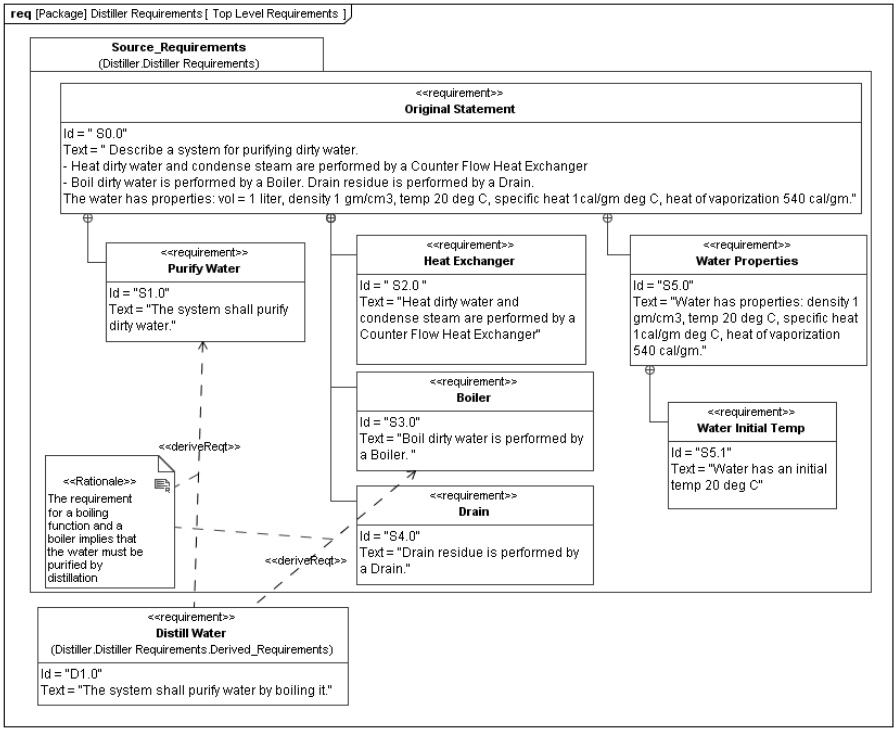
\includegraphics[width=0.65\linewidth]{Resources/4_sysml_req_diagram.png}
	\caption{Example SysML Requirements Diagram.}
	\label{fig:sysml_req_diagram}
\end{figure} 

\clearpage
\subsection*{Communication Diagram \cite{communication_diagram}}
Models the communication between objects. Connections are used to represent the need for communication during execution between objects.
\begin{itemize}
	\item[\textbf{+}] Messages are grouped for easy repositioning.
	\item[\textbf{+}] Use swimlanes to represent layers of a system.
	\item[\textbf{+}] See where trade-offs need to be made.
	\item[\textbf{-}] Low level.
\end{itemize}

Example:\\
Can be used for modelling the interaction of the user with the UI and the system (Figure \ref{fig:communication_diagram}). Or for modelling the inter system communications. This could be used to test the requirements.
\begin{figure}[h]
	\centering
	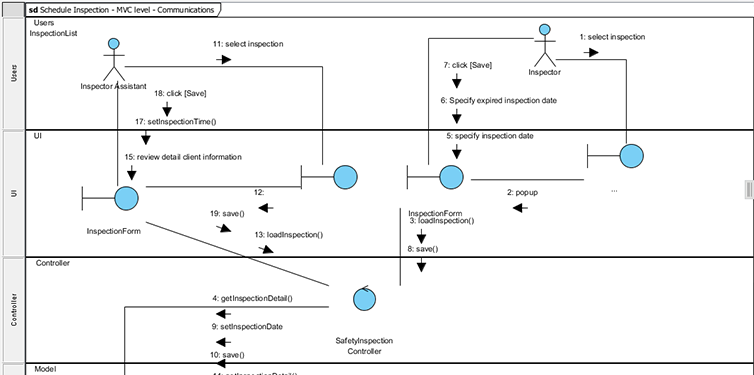
\includegraphics[width=1\linewidth]{Resources/4_communication_diagram.png}
	\caption{Example communication diagram.}
	\label{fig:communication_diagram}
\end{figure} 

\clearpage
\subsection*{Process life-cycle diagram \cite{sysml}}
Used to model the life-cycle of sub-processes to parent processes.
\begin{itemize}
	\item[\textbf{+}] Communicate the life-cycle of processes within the business and possibly with stakeholders.
	\item[\textbf{+}] Could also be used to model the life-cycle of system processes.
	\item[\textbf{-}] Seems more appropriate to model business process than requirements/system processes.
	\item[\textbf{-}] Does not model any data.
\end{itemize}

Example:\\
See Figure \ref{fig:lifecycle_diagram}, sub-processes are grouped within the life-cycle of parent-processes.
\begin{figure}[h]
	\centering
	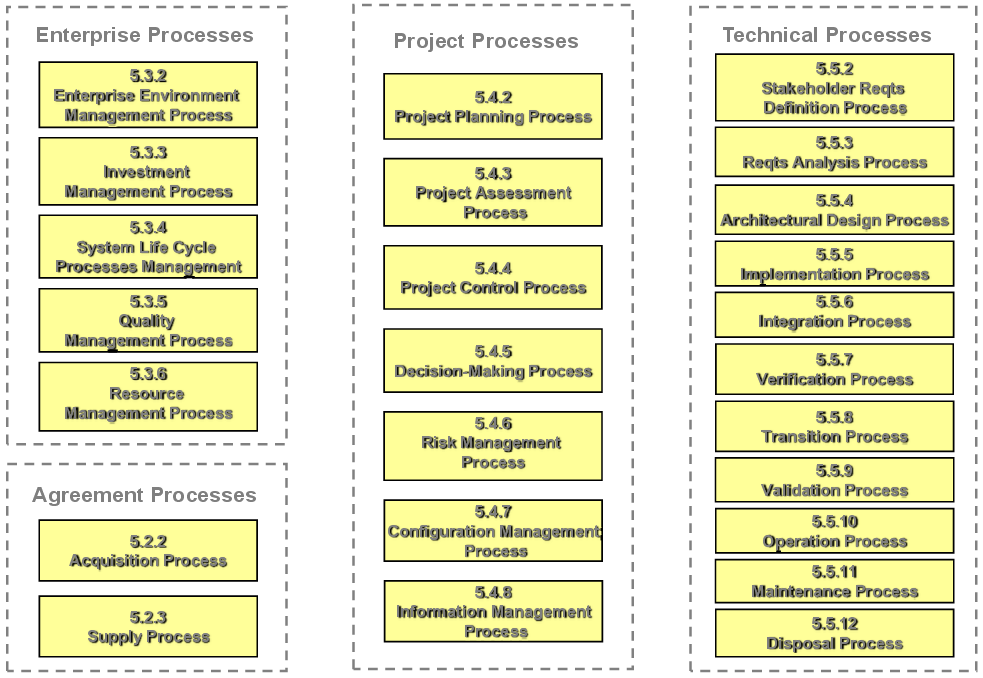
\includegraphics[width=1\linewidth]{Resources/4_lifecycle_diagram.png}
	\caption{Example process life-cycle diagram.}
	\label{fig:lifecycle_diagram}
\end{figure} 


\clearpage
\section*{4.1}
Good models for organizing the knowledge about the successor of Blackboard would be:
\begin{itemize}
	\item Sysml requirements diagram
	\item Dependency diagram
	\item System context diagram
	\item Decision trees
	\item Goal/requirements trees
\end{itemize}
All these model either dependencies between requirements, knowledge and decisions, or the scoping of (sub)systems. They can be used to reason about knowledge or about the requirements of the system-to-be. \emph{ps: this is off course, by any means, not an exhaustive list..}


\section*{4.2}
With the system proposed by Axel van Lamsweerde \cite{lamsweerde} you cannot quickly restructure your data per se. But new knowledge and insights could be added to their respective knowledge base which would make it easy to see what parts are affected by this new data.

By grouping certain types of knowledge together, such as domain understanding through research or knowledge acquired from elicitations. This knowledge is then evaluated and negotiated and this in turn derives the system specification and documentation (requirements).

Whenever new data is added to the knowledge phase, the impact of this could be observed in the evaluation and negotiation phase and the requirements would be changed as a result if needed. If you stick to this scheme you remove the need to restructure your data, as the effects of new knowledge and insights follow a clear and predictable path all the way down to the requirements.

\chapter{References}

\begin{thebibliography}{9}
	
	\bibitem{req_en_book}
	Joao M. Fernandes, Ricardo J. Machado, \\
	\emph{Requirements in Engineering Projects}
	
	\bibitem{sysml}
	OMG Systems Modeling Language (OMG SysML) \\
	\url{http://www.omgsysml.org/INCOSE-OMGSysML-Tutorial-Final-090901.pdf}
	
	\bibitem{communication_diagram}
	\url{http://www.visual-paradigm.com/features/uml-and-sysml-modeling/}
	
	\bibitem{lamsweerde}
	Axel van Lamsweerde, \\
	\emph{Requirements Engineering, From System Goals to UML Models to Software Specifications}
	
\end{thebibliography}


\appendix


\end{document}
